%!TeX root=MemoriaTFG.tex
\chapter{Disseny de la solució}\label{disseny}
En aquest capítol es veurà quina ha estat la sol·lució al problema analitzat a l'apartat anterior. Es tracta de desenvolupar una \ac{API} que permeti als integrant de la comunitat universitaria gaudir d'un servei de missatgeria. Aquesta \ac{API} ha de servir de suport a diferents clients (aplicacions d'escriptori, aplicacions mòbils o aplicacions web entre d'altres). \\

En primer lloc s'exposa una visió global de les parts de l'aplicació. A continuació es farà una explicació detallada de cada mòdul de l'aplicació. S'ha dividir l'aplicació en els següents mòduls: 
\begin{itemize}

	\item \textbf{Model de dades:} s'explicarà com s'ha estructurat el model de dades replicat.
	\item \textbf{Serveis:} s'explicarà l'arquitectura \ac{SOA}, com s'ha estructurat, els diferents serveis que s'han desenvolupat i llibreries per donar suport a aquests.
	\item \textbf{\ac{API}:} s'explicarà com s'ha estructurat l'\ac{API} que s'ha dissenyat. En aquest apartat també s'explicarà com s'han definit i implementat els nivells d'accés als recursos de l'\ac{API}.
	\item \textbf{Integració contínua:} s'explicarà com s'han elaborat els tests unitaris per comprovar el correcte funcionament de l'aplicació. També s'explicarà el funcionament del servei \textbf{Travis CI} per a assegurar que cada desplegament a producció no altera el correcte funcionament del servei.
	
\end{itemize}

Una descripció a alt nivell de l'estructura de l'aplicació sería la següent: quan es fà una petició a l'\ac{API}, aquesta crida a un determinat servei que de manera abstracta realitza operacions sobre les dades (lectura o escriptura) residents a la base de dades. Una vegada fetes les operacions sobre la base de dades, el resultat d'aquesta es serialitza i l'\ac{API} s'encarrega de mostrar les dades a l'usuari. Es pot veure aquesta estructura a la figura \ref{fig:estructura}.

\begin{figure}[h!]
    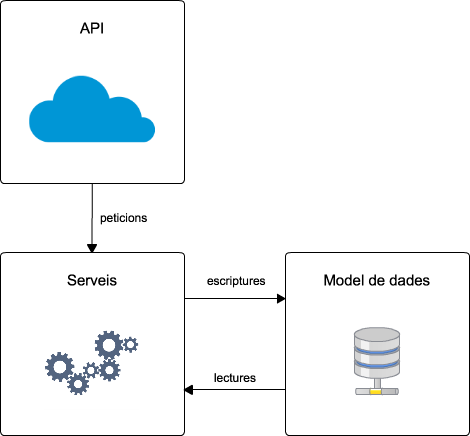
\includegraphics[scale=0.7]{img/estructura.png}
    \centering
    \caption{Visió global de com es connecten els tres principals mòduls de l'aplicació}
    \label{fig:estructura}
\end{figure}

\section{Model de dades}
Per preservar la independència de les dades del nostre sistema de les dades de la universitat, s'ha decidit replicar les dades necessàries al nostre sistema per no operar directament sobre el conjunt de dades de la universitat, per no dependre de la estructura que manté la universitat i per no alterar el rendiment dels sistemes de la universitat.\\

S'ha dissenyat una estructura de dades de manera que no depengui de cap universitat i pugui ser usada per qualsevol institució educativa. A la figura \ref{fig:model} es pot veure el model de dades resultant. \\

\begin{figure}[here]
    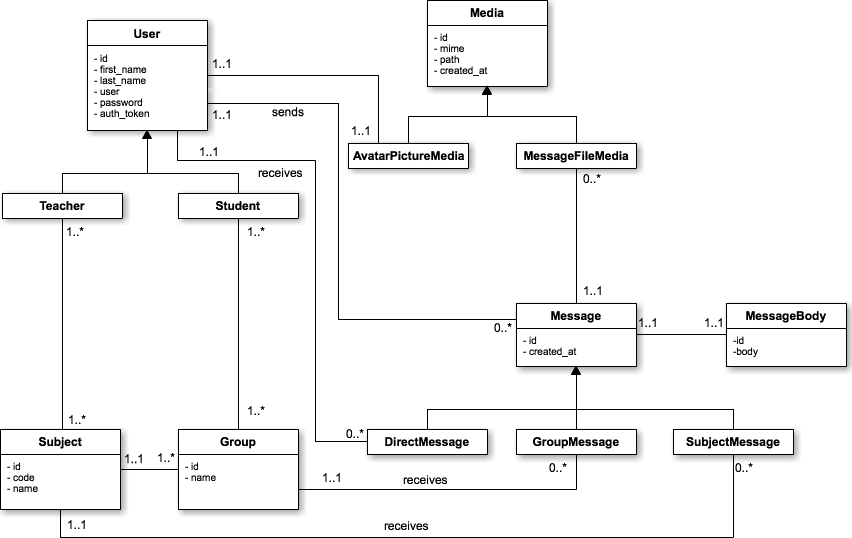
\includegraphics[scale=0.5]{img/uml.png}
    \centering
    \caption{Model de dades}
    \label{fig:model}
\end{figure}

Les entitats del model dissenyat són les següents: usuari, professor, estudiant, assignatura, grup, missatge, cos del missatge, missatge directe, missatge de grup, missatge d'assignatura, fitxer, avatar de l'usuari i fitxer de missatge. A continuació s'explicarà cada entitat del model. Per tancar la secció veurem com funciona el \emph{querier} de \emph{SQLAlchemy}, com s'elaboren consultes les consultes de manera abstracta.

	\subsection{Usuari, professor i estudiant} \label{usuari_professor_estudiant}

	L'entitat \texttt{User} representa qualsevol usuari que interactuï amb l'\ac{API}. Un usuari està composat pels següents camps: 
	\begin{itemize}
		\item \textbf{id:} identificador únic de l'usuari. És un camp numèric i auto incremental.
		\item \textbf{first\_name:} nom de l'usuari.
		\item \textbf{last\_name:} cognoms de l'usuari.
		\item \textbf{user:} usuari d'accés al sistema. S'ha decidit per defecte s'intenti que aquest coincideixi amb les credencials d'accés a l'intranet de la universitat que implementi el servei.
		\item \textbf{password:} contrassenya d'accés al sistema. S'ha decidit que per defecte s'intenti que aquesta coincideixi amb la mateixa de les credencials d'accés a la intranet de la universitat que implementi el servei. 
		\item \textbf{auth\_token:} token d'autorització al sistema. S'explica amb més detall a la secció %TODO.
	\end{itemize}
	
	Com es veu al diagrama de classes del model de dades (figura \ref{fig:model}), les entitats Professor i Estudiant hereden de l'entitat \texttt{User}. No hi ha cap diferència en els atributs de les entitats filles d'Usuari, a la pràctica s'ha afegit un atribut de típus enter que diferencia si un usuari és professor o alumne. Es ampliable a nous tipus (per exemple: un administrador, \ac{PAS}, etc...). \\
	
	Per implementar aquesta distinció entre professor i alumne, amb l'ajut de SQLAlchemy s'ha creat l'entitat \texttt{UserType}. L'entitat \texttt{UserType} representa els diferents típus d'usuari que hi pot haver en el sistema. En el nostre cas representarà o bé un professor o bé un alumne. Com es pot veure a la figura \ref{fig:entitats_usuari} l'entitat \texttt{User} té una clau forana a \texttt{UserType}, d'aquesta manera relacionam l'usuari amb el seu tipus. \\
	
	Un altre aspecte a destacar de l'entitat \texttt{User} és el token d'autorització al sistema. Aquest aspecte s'explicarà en l'apartat \ref{sec_api2}.
	
\begin{figure}[here]
	\begin{python}
	class UserType:
	
    	TEACHER = 1
    	STUDENT = 2

    	id = Column(Integer, primary_key=True)
    	name = Column(String(15))
    	
	class User:
	
    	id = Column(BigInteger, primary_key=True)
    	first_name = Column(String(60))
    	last_name = Column(String(120))

    	user = Column(String(32), unique=True)
    	password = Column(String(256))
   		auth_token = Column(String(64))
    	type_id = Column(Integer, ForeignKey('user_type.id'))
    	type = relationship(UserType, backref=backref('users', uselist=True, cascade='delete,all'))
    	
    	def is_teacher(self):
    		return self.type.id == UserType.TEACHER
    		
    	def is_student(self):
    		return self.type.id == UserType.STUDENT
	\end{python}
    \caption{Entitats d'usuari, professor i alumne}
    \label{fig:entitats_usuari}
\end{figure}

	\subsection{Media, avatar i fitxer de missatge} \label{media_avatar_fitxer}
	L'entitat \texttt{Media} representa el contingut multimèdia que un usuari pot publicar al servei. Es distingeix entre un avatar i un fitxer de missatge. Un avatar és la fotografia de perfil de l'usuari i un fitxer de missatge és un fitxer que pertany a un únic missatge. \\
	
	Una entitat \texttt{Media} està composada pels següents atributs:
	
	\begin{itemize}
		\item \textbf{id:} identificador únic de l'element multimèdia.
		\item \textbf{type:} tipus de multimèdia. S'explicarà a continuació.
		\item \textbf{mime:} típus \ac{MIME} del fitxer.
		\item \textbf{path:} ruta del fitxer físic al sistema de fitxers del servidor.
		\item \textbf{created\_at:} \emph{timestamp} de creació del fitxer.
	\end{itemize}
	
	En aquest cas, la diferència entre els dos típus de multimèdia és l'entitat del nostre sistema amb la que estàn relacionats. En el cas d'un avatar d'usuari aquest es relaciona amb l'usuari, en el cas d'un fitxer de missatge es relacionara amb un missatge.\\

	Una pregunta que es pot formular el lector és per què s'ha creat una entitat per l'avatar de l'usuari si aquest podria ser un atribut de l'entitat Usuari (veure seccio \ref{usuari_professor_estudiant}). La resposta a aquesta pregunta és per tenir la mateixa interfície d'accés als avatars d'usuari que als fitxers multimèdia. Ambdos típus de multimèdia es comportaràn de la mateixa manera i amb aquesta implementació tenim tot el contigut multimèdia centralitzat en una única entitat.	\\
	
	\emph{SQLAlchemy} ens brinda la oportunitat de fer ús de l'herència a l'hora de crear entitats. Per implementar-ho s'han creat les següents entitats: \texttt{Media}, \texttt{AvatarMedia} i \texttt{MessageFileMedia}. L'entitat \texttt{AvatarMedia} té una clau forana cap a l'entitat \texttt{User} (veure secció \ref{usuari_professor_estudiant}), mentre que l'entitat \texttt{MessageFileMedia} te la clau forana cap a l'entitat \texttt{Message} (veure secció \ref{missatge_directe_grup_assignatura}). Es pot veure el codi de les tres entitats a la figura \ref{fig:entitats_multimedia}. \\
	

\begin{figure}[p]
	\begin{python}
class MediaType:
	
	AVATAR = 1
	MESSAGE_FILE = 2
		
	id = Column(Integer, primary_key=True)
	name = Column(String(20))
    	
class Media:

    id = Column(BigInteger, primary_key=True)
    type = Column(Integer, ForeignKey('media_type.id'))
    mime = Column(String(64))
    path = Column(String(256))
    created_at = Column(DateTime)

    __mapper_args__ = {'polymorphic_on': type}

class AvatarMedia(Media):
	
    user_id = Column(BigInteger, ForeignKey('user.id'), unique=True)
    user = relationship(User,  backref=backref('avatar', uselist=True, cascade='delete,all'))

    __mapper_args__ = {'polymorphic_identity': MediaType.AVATAR}

class MessageFileMedia(Media):

    message_id = Column(BigInteger, ForeignKey('message.id'))
    message = relationship(backref=backref('media', uselist=True, cascade='delete,all'))

    __mapper_args__ = {'polymorphic_identity': MediaType.MESSAGE_FILE}
    	
	\end{python}
    \caption{Entitats multimedia}
    \label{fig:entitats_multimedia}
\end{figure}
   
    Al igual que hem fet amb l'entitat \texttt{User}, amb l'entitat \texttt{Media} també hem definit una entitat auxiliar: \texttt{MediaType}. Aquesta entitat auxiliar ens servirà per diferenciar entre els dos típus de contingut multimèdia que tenim. El seu comportament és el mateix que l'entitat \texttt{UserType} explicada anteriorment.\\
    
    Com que entre les dues entitats filles de \texttt{Media} si que hi ha diferència, en aquest cas s'ha optat per usar la herència que ens brinda la \ac{POO}. A nivell de llenguatge de programació s'ha fet que les classes \texttt{AvatarMedia} i \texttt{MessageFileMedia} heretin de \texttt{Media}.\\
    
     A nivell de base de dades, s'ha d'indicar a l'\ac{ORM} quin camp de l'entitat pare ha d'usar per discriminar entre ambdos típus de multimèdia. És en aquest punt on entra en joc l'entitat \texttt{MediaType}. Si ens fixam en el codi de la figura \ref{fig:entitats_multimedia} podem veure com les dues entitats filles de \texttt{Media} tenen l'atribut \texttt{\_\_mapper\_args\_\_}. Aquest atribut defineix, entre d'altres, quin valor ha de tenir l'atribut \texttt{type} per que es pugui distingir una entitat de l'altra.\\
    
    Un altre aspecte a destacar del codi dels models són les relacions a les classes filles. Es pot observar que tant l'entitat \texttt{AvatarMedia} i \texttt{MessageFileMedia} tenen dos atributs cada una. Per una banda \texttt{AvatarMedia} te \texttt{user\_id} i \texttt{user}, per l'altra banda, l'entitat \texttt{MessageFileMedia} te \texttt{message\_id} i \texttt{message}. \\
    
    En ambdos casos, el primer es la clau forana cap a l'entitat que correspongui (\texttt{User} en el cas d'\texttt{AvatarMedia} i \texttt{Message} en el cas de \texttt{MessageFileMedia}). El segon atribut representa l'entitat a la qual fan referència. Si tenim una entitat \texttt{AvatarMedia} amb \texttt{user\_id = 1}, el valor de \texttt{user} serà l'usuari amb \texttt{id = 1}.\\
   
    \subsection{Missatge, directe, de grup, d'assignatura i cos del missatge}\label{missatge_directe_grup_assignatura}
    
    L'entitat \texttt{Message} representa qualsevol típus de missatge, ja sigui directe, a un grup o a una assignatura. A continuació es pot veure una relació dels atributs de l'entitat missatge:
    
    \begin{itemize}
    	\item \textbf{id:} identificador únic del missatge.
    	\item \textbf{type:} típus de missatge. El seu funcionament és el mateix que el típus multimèdia explicat a la secció \ref{media_avatar_fitxer}.
    	\item \textbf{sender\_id:} identificador de l'usuari que envia el missatge. 
    	\item \textbf{body\_id:} identificador del cos del missatge. S'explicarà amb més detall a continuació.
    \end{itemize}
    
     Aquesta entitat també fa ús de l'herència que ens brinda la \ac{POO}. En aquest cas, hem de distingir tres típus de missatge: \texttt{DirectMessage}, \texttt{GroupMessage} i \texttt{SubjectMessage}. Tots tres típus de missatge tenen com a remitent un usuari, ja sigui professor o alumne. \\
     
     Un missatge directe va dirigit a un usuari, un missatge de grup va dirigit a un grup d'assignatura i un missatge d'assignatura va dirigit a una assignatura, al que anomenarem fòrum general de l'assignatura. \\
    
   	La implementació de l'herència és la mateixa que la que s'ha usat per l'entitat \texttt{Media} (veure secció \ref{media_avatar_fitxer}) i no entrarem en detall de la seva implementació. També és fa us de la tècnica \texttt{relationship} que ens relaciona la clau forana amb l'entitat que correspon. \\
   	
   	L'entitat \texttt{DirectMessage} conté una clau forana cap a usuari que referencia l'usuari al qual s'ha enviat el missatge. \\
   	
   	L'entitat \texttt{GroupMessage} conté una clau forana cap al grup que referencia el grup al qual s'ha enviat el missatge.\\
   	
   	 L'entitat \texttt{SubjectMessage} conté una clau forana cap a l'assignatura que referencia l'assignatura a la qual s'ha enviat el missatge.\\
   
   	Per una altra banda, s'ha creat l'entitat \texttt{MessageBody} que representa el contingut del missatge. S'ha definit una longitud màxima d'aquest de quatre-cents caràcters. Al ser el cos del missatge de longitud variable, cada registre tendrà un tamany variable i quedaràn espais de memòria reservats per el cos del missatge buits al disc. Per aquest motiu s'ha traslladat el contigut del missatge a una entitat apart i així l'entitat \texttt{Message} queda més compactada i fora espais de memoria buits.\\
   	
   	\subsection{Assignatura i grup}
   	
   	L'entitat \texttt{Subject} representa qualsevol assignatura que es pugui impartir dins la universitat. Una assignatura està composada pels següents atributs:
   	
   	\begin{itemize}
   		\item \textbf{id:} identificador únic de l'assignatura.
   		\item \textbf{code:} codi unic de l'assignatura, si escau.
   		\item \textbf{name:} nom de l'assignatura.
   	\end{itemize}
   	
   	L'entitat \texttt{Group} representa qualsevol grup que pertanyi a una assignatura que es pugui impartir dins la universitat. Un grup està composat pels següents atributs:
   	
   	\begin{itemize}
   		\item \textbf{id:} identificador únic del grup.
   		\item \textbf{nom:} nom del grup.
   		\item \textbf{subject\_id:} identificador de l'assignatura que el grup pertany. 
   	\end{itemize}
   	
   	Segons el model de dades (veure figura \ref{fig:model}) un grup pertany només a una assignatura. Per aquest motiu l'entitat \texttt{Group} conté una clau forana cap a l'entitat Assignatura.\\
   	
   	S'han creat dues entitats auxiliars, \texttt{TeacherSubject} i \texttt{StudentGroup}. La primera fà referència a la relació entre professor i assignatura. En aquesta entitat es poden trobar els següents atributs:
   	
   	\begin{itemize}
   		\item \textbf{teacher\_id:} identificador del professor. A la pràctica fà referència a un identificador d'usuari.
   		\item \textbf{subject\_id:} identificador de l'assignatura.
   	\end{itemize}
   	
   	Ambdos atributs actúen com a clau primària de la taula, per aquest motiu no és necessàri tenir un atribut \texttt{id} que actuï com a tal. El mateix fenòmen succeeix a l'entitat \texttt{SubjectGroup}, que té els següents atributs:
   	
   	\begin{itemize}
   		\item \textbf{student\_id:} identificador de l'alumne. A la pràctica fa referència a un identificador d'usuari.
   		\item \textbf{group\_id:} identificador del grup.
   	\end{itemize}
   	   
   \subsection{\emph{Querier} de \emph{SQLAlchemy}}
   
   El \emph{querier} de \emph{SQLAlchemy} serveix per a realitzar consultes a la base de dades sense fer ús del llenguatge \ac{SQL}. Definiex una manera abstracta d'obtenir, inserir, actualitzar i eliminar registres de la base de dades, idependentment del \ac{SGBD} que s'estigui empleant. \\
  
	A la figura \ref{fig:exemples_consultes} es poden veure uns quants exemples de consultes fetes amb el \emph{querier} de \emph{SQLAlchemy}. Aquestes seràn explicades a continuació:

\begin{figure}
  	\begin{python}
# 1- Tots els usuaris
all_users = db.query(User).all()

# 2- Usuari amb l'id 5
user = db.query(User).get(5)

# 3- Els tres darrers usuaris inserits a la taula 
last_three_users = db.query(User).\
				order_by(User.id.desc()).\
				limit(3).all()

# 4- Usuaris amb nom 'Joan'
users_with_name_joan = db.query(User).\
				filter(User.first_name == 'Joan').all()
											
# 5- Usuaris matriculats a l'assignatura amb id 3
users_of_subject_3 = db.query(User).\
				join(StudentGroup, User.id == StudentGroup.student_id).\
				join(Group, StudentGroup.group_id == Group.id).\
				join(Subject, Group.subject_id == Subject.id).\
				filter(Subject.id == 3).all()
				
	\end{python}
	\caption{Exemples de consultes}
	\label{fig:exemples_consultes}
\end{figure}

	\begin{enumerate}
		\item Consulta que obté tots els usuaris de l'entitat \texttt{User}. La funció del \emph{querier} \texttt{all} obté tots els registres.
		
		\item Consulta que obté l'usuari amb identificador 5. La funció del \emph{querier} \texttt{get} obté un registre de la taula a partir de la seva clau primària. En aquest la clau primària de la taula usuari és l'identificador únic d'aquest.
		
		\item Consulta que obté els tres darrers usuaris inserits a la taula. La funció \texttt{order\_by} estableix per quina (o quines) columnes s'ha d'ordenar la consulta. Aquesta funció accepta tants paràmetres com l'usuari vulgui. Els seus paràmetres han de ser del format \texttt{Entitat.propietat.asc()} o \texttt{Entitat.propietat.desc()} per ordenar de forma ascendent o descendent. L'altre funció que apareix en aquesta consulta és \texttt{limit} que estableix el màxim de registres que pot tornar la consulta.
		
		\item Consulta que obté tots els usuaris que com a nom tenen "Joan". Apareix per primer cop la funció \texttt{filter}. Aquesta accepta múltiples paràmetres, tants com l'usuari vulgui, en format de condicionals de Python. Es poden utilitzar tots els operadors disponibles al llenguatge.
		
		\item Consulta que obté tots els usuaris matriculats a l'assignatura amb identificador 3.Apareix per primer cop la funció \texttt{join} que actúa com el \texttt{JOIN} de \ac{SQL}. Com a primer paràmetre de la funció hem d'especificar amb quina taula volem el producte cartesià i en segon lloc amb quins paràmetres de cada taula l'hem de relacionar.
		
	\end{enumerate}
	
	Cada consulta realitzada sobre una entitat retorna instàncies d'aquesta entitat. Si la consulta retorna més d'un registre rebrem una llista d'entitats. En el cas de que volguem obtenir només un registre ens retornarà una instancia de l'entitat demanada.

  
\section{Serveis}
	Fins ara hem vist com està composat el model de dades de la nostra aplicació. Hem vist les diferents entitats que té i com es relacionen entre sí. En aquest apartat es veurà el principal component de l'aplicació. Es tracta dels serveis de l'aplicació, que no són més que petits components que interactúen amb la base de dades mitjançant l'\ac{ORM} i que tenen una única responsabilitat sobre les dades. \\
	
	En aquesta secció en primer lloc es veurà la interfície dissenyada per a la construcció de serveis. En segon lloc veurem la llibreria de validació que s'ha desenvolupat per donar suport a la invocació de serveis. Per finalitzar, s'explicaràn els serveis desenvolupats, separats les següents responsabilitats:
	
	\begin{itemize}
		\item \textbf{Usuari}
		\item \textbf{Multimèdia}
		\item \textbf{Missatge}
		\item \textbf{Assignatura}
		\item \textbf{Grup}
	\end{itemize}
	
	\subsection{Interfície}
	
	Un dels principis del \ac{SOA} (veure secció \ref{soa}), és que els serveis tenen un acord de comunicació comú entre ells i que tots els serveis són invocats de la mateixa manera. Sigui quin sigui el servei, s'invocarà de la mateixa manera.\\
	
	A nivell de llenguatge, un servei està implementat dins una classe amb tres mètodes: un contracte d'entrada, una funció d'execució i un contracte de sortida. Abans de l'execució del servei es fa una validació del contracte d'entrada. Aquesta validació s'explicarà a la secció \ref{validacio}.\\
	
	 A la figura \ref{fig:servei} podem trobar els elements que intervenen a un servei.\\
	
	\begin{figure}[h!]
		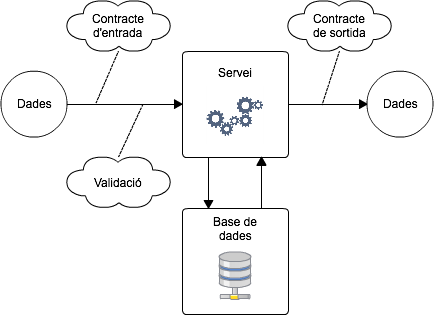
\includegraphics[scale=0.5]{img/servei.png}
   		\centering
    	\caption{Elements que intervenen a un servei}
   	 	\label{fig:servei}
	\end{figure}
	
	L'esquelet d'un servei està definit per tres principals funcions, aquest es pot veure a la figura \ref{fig:esquelet_servei}. Aquestes tres funcions són les següents:
	
	\begin{itemize}
		\item \textbf{input:} definieix el contracte d'entrada del servei. Aquesta funció ha de retornar un diccionari amb els paràmetres que pot acceptar el servei com a claus del diccionari, i el valor de cada clau serà el seu validador que li correspon.
		 
		\item \textbf{output:} defineix el contracte de sortida del servei. Aquesta funció ha de retornar una altra funció que evalui si el resultat de l'execució del servei és el correcte o no. Aquesta funció rebrà com a paràmetre el resultat de l'execució del servei.
		
		\item \textbf{execute:} funció d'execució de servei. Reb com a paràmetre un diccionari que té com a claus el nom dels arguments i com a valor de la clau, el valor de l'argument.
	\end{itemize}
	
	\begin{figure}[h!]
		\begin{python}
class MyService:
	
	# Contracte d'entrada
	def input(self):
		return {}
	
	# Contracte de sortida
	def output(self):
		return lambda x: pass
		
	# Funcio d'execucio
	def execute(self, args):
		pass
		\end{python}
		\caption{Esquelet d'un servei}
		\label{fig:esquelet_servei}
	\end{figure}
	
	El fluxe d'execució d'un servei és el següent: quan s'invoca un servei el primer que es fa es comprovar que els arguments que se li han passat concorden amb els especificats al contracte d'entrada.  En aquesta comprovació poden succeïr dues coses: per una banda, que passem un paràmetre no especificat al contracte d'entrada o que no passem un paràmetre requerit. En ambdos casos es notificarà a l'usuari amb una excepció. En el primer cas l'excepció no serà capturada per cap entitat superior ja que es considerat un error greu de programació. En el segon cas, l'excepció serà capturada i gestionada per una entitat superior que informarà a l'usuari de l'error. Aquest tractament es veurà a la secció \ref{sec_api2}.\\
	
	Una vegada feta la comprovació del contracte d'entrada, el següent pas és netejar els paràmetres. Es considerarà la neteja de paràmetres com a la conversió al tipus que el validador espera.\\
	
	Python és un llenguatge no tipat, és a dir, no hi ha típus per a les variables. En un moment de l'execució una variable pot ser de típus enter i en un altre moment ser de típus llista. És per aquest motiu que si un paràmetre del contracte d'entrada espera un valor de típus enter i per a qualsevol motiu el valor passat és l'enter pero dins una cadena de text, el procés passarà aquesta cadena de text a enter mitjançant les funcions de \emph{casting} del llenguatge.\\
	
	Aquesta conversió pren força quan els arguments venen directament d'una petició \ac{HTTP}, on la que les variables no estan tipades. Quan la variable arribi al servei, si parlam del cas d'un nombre enter, es farà la conversió de cadena de text a enter. \\
	
	Si aquesta neteja de paràmetres falla, és a dir, el tipus esperat pel validador no és el de la variable. Es notificarà a mitjançant una excepció a l'usuari. Aquest tractament d'errors també es veurà a la secció \ref{sec_api2}.\\

	Una vegada feta la neteja de paràmetres i la comprovació de típus, és el moment d'executar el servei. S'executarà el codi de dins la funció \texttt{execute}. Cal recordar que aquesta funció que el programador ha d'implementar, reb com a únic argument els paràmetres netjats en un diccionari amb el format comentat anteriorment.\\
	
	Una vegada feta l'execució de la funció, el seu resultat es passarà a la funció especificada dins el contracte de sortida del servei. Aquesta funció reb un únic paràmetre que és el resultat de la funció \texttt{execute} i ha de retornar vertader o fals en funció de si el resultat és l'esperat o no.\\
	
	A la figura \ref{fig:fluxe} es pot observar el diagrama de fluxe d'execució d'un servei. 
	
	\begin{figure}[h!]
		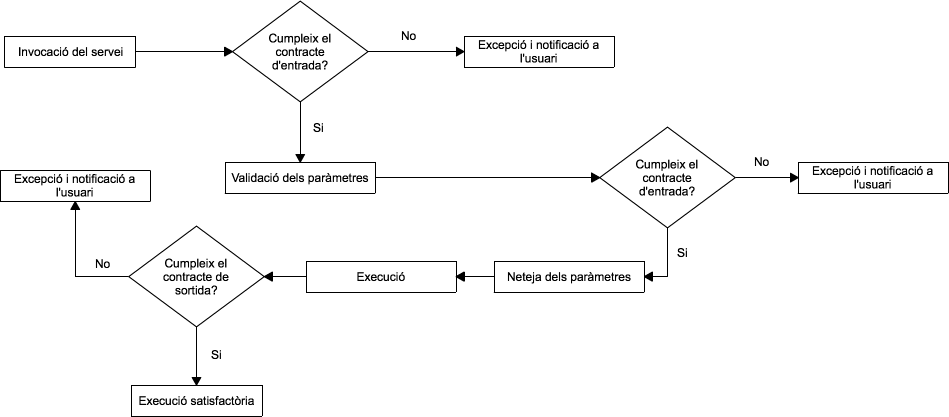
\includegraphics[scale=0.35]{img/flux.png}
		\label{fig:fluxe}
		\caption{Diagrama del fluxe d'execució d'un servei}
	\end{figure}
	
	Podem veure l'exemple d'un servei a la figura \ref{fig:ex_servei}. Aquest senzill servei d'exemple reb com a paràmetre dos nombres enters i retorna el seu producte. 
	
	\begin{figure}[h!]
		\begin{python}
class Multiplication:
	
	# Contracte d'entrada
	def input(self):
		return {
			'a': IntegerValidator({'required': True}),
			'b': IntegerValidator({'required': True})
		}
	
	# Contracte de sortida
	def output(self):
		return lambda x: isinstance(x, int)
		
	# Funcio d'execucio
	def execute(self, args):
		a = args.get('a')
		b = args.get('b')
		return a * b
		\end{python}
		\caption{Servei d'exemple}
		\label{fig:ex_servei}
	\end{figure}
	
	Fins ara hem vist la forma en que es declara i s'implementa un servei. Es pot observar un exemple d'invocació d'un servei a la figura \ref{fig:invocacio_servei}. \\
	
		\begin{figure}[h!]
		\begin{python}
multiplication_service = Multiplication()
result = multiplication_service.call({
	'a': 3,
	'b': 6
})
print result
>>> 18
		\end{python}
		\caption{Invocació d'un servei}
		\label{fig:invocacio_servei}
	\end{figure}
	
	Cal destacar que el mètode que es pot observar a la figura \ref{fig:invocacio_servei}, \texttt{call} no es troba implementat al nostre servei \texttt{Multiplication}. Tots els serveis extenen d'una entitat anomenada \texttt{BaseService} que conté, apart del mètode \texttt{call}, altres mètodes auxiliars per donar suport a l'execució. Aquest mètodes auxiliars inclouen la comprovació de que els paràmetres introduïts durant la invocació concorden amb els declarats al contracte d'entrada, la comprovació del contracte de sortida, entre d'altres.\\
	
	En el nostre cas, la majoria dels serveis interactuaràn amb la base de dades. Aquests serveis, enlloc d'extendre de la classe \texttt{BaseService}, extendràn d'una entitat \texttt{BasePersistanceService}, filla de \texttt{BaseService}, que tendrà com a atribut la sessió a la base de dades.

	\subsection{Llibreria de validació} \label{validacio}
	
	Com ja s'ha comentat a la secció anterior, els serveis venen acompanyats d'una llibreria auxiliar de validació. Entenem per validador una entitat que s'encarrega de validar la correctesa d'una variable. Aquesta validació pot anar per exemple desde una simple comprovació de típus fins a la correctesa del format de una \ac{URL}. \\
	
	S'ha dissenyat una interfície de validació per donar suport tant a la validació dels serveis com a la validació dels paràmetres de les peticions \ac{HTTP}.\\
	
	Un validador consta de dos elements principals. El primer és una funció per comprovar que el valor cumpleix els requisits especificats. En cas de validació invàlida, aquesta funció establirà els errors corresponents. En cas de validació satisfactòria no la funció no alterarà l'estat del validador.\\
	
	L'altre element fonamental dels validadors és la funció de neteja del valor. Aquesta nomes s'invocarà en el cas de validació satisfactòria.  A la figura \ref{fig:int_validador} podem veure un exemple de validador de nombres enters.\\
	
	\begin{figure}[h!]
		\begin{python}
class IntegerValidator:

	def check_value(self, value):
		try:
			int(value)
		except ValueError:
			self.add_error('The value is not an integer')
			
	def clean_value(self, value):
		return int(value)
		\end{python}
		\caption{Validador de nombres enters}
		\label{fig:int_validador}
	\end{figure}	
	 
	 Com passa amb els serveis, els validadors hereten d'una entitat anomenada \texttt{BaseValidator} que conté mètodes auxiliars per donar suport a la validació. El mètode a destacar d'aquesta entitat és el \texttt{validate}. Aquest mètode engloba les dues principals funcions dels validadors. En primer lloc comprova els errors, si n'hi ha tira una excepció que sera capturada per una entitat superior (aquest aspecte es veurà a la seccio \ref{sec_api2}). En cas de validació satisfactòria, es neteja i converteix al tipus del validador i es retorna el valor netejat.
	 
	 Un darrer aspecte a destacar dels validadors són les seves opcions. Al inicialitzar el validador se li poden passar una sèrie d'opcions. Per defecte tots els validadors tendràn les següents opcions:
	 
	 \begin{itemize}
	 	\item \textbf{required:} booleà que indicarà si obligatoriament s'ha de passar un valor o no.
	 	\item \textbf{default:} valor per defecte del validador en el cas de que no se'n passi cap.
	 \end{itemize}
	 
	 Aquestes dues opcions estan especificades al \texttt{BaseValidator} i es poden extendre a cada validador específic.
	 
	\subsection{Serveis de l'aplicació} \label{serveis_aplicacio}
	
		En el capítol anterior s'ha exposat la manera en que s'implementen els serveis. Hem vist en que consisteix el contracte d'entrada, el contracte de sortida, la funció d'execució del servei i la llibreria auxiliar per donar suport a la validació del contracte d'entrada.\\
		
		En aquesta secció es veuràn els principals serveis desenvolupats per l'aplicació. Aquests serveis els hem dividit en mòduls segons la seva responsabilitat. Aquests mòduls són els següents:
		
		\begin{itemize}
			\item \textbf{Usuari:} serveis que operen amb l'entitat Usuari.
			\item \textbf{Multimèdia:} serveis que gestionen contingut multimèdia.
			\item \textbf{Missatge:} serveis que operen amb l'entitat Missatge.
			\item \textbf{Assignatura:} serveis que operen amb l'entitat Assignatura.
			\item \textbf{Grup:} serveis que operen amb l'entitat Grup.
		\end{itemize}
		\subsubsection{Usuari}
			
		Els serveis d'usuari són els que operen damunt l'entitat Usuari. D'aquesta secció de serveis podem destacar-ne els següents:
		
		\begin{itemize}
			\item \textbf{GetUser:}: servei que obté un usuari.
				\begin{itemize}
					\item \textbf{Contracte d'entrada}
						\begin{itemize}
							\item \textbf{user\_ud:} identificador de l'usuari.
						\end{itemize}
					\item \textbf{Contracte de sortida:} entitat \texttt{User} o res (en el cas de que l'usuari no existeixi).
				\end{itemize}
		
			\item \textbf{GetSubjectTeachers:}: servei que obté els professors d'una assignatura. Si observam el model de dades només s'ha de consultar amb quines assignatures està relacionat el professor.
				\begin{itemize}
					\item \textbf{Contracte d'entrada}
						\begin{itemize}
							\item \textbf{subject\_id:} identificador de l'assignatura de la qual es volen consultar els professors.
						\end{itemize}
					\item \textbf{Contracte de sortida:} llista d'entitats \texttt{User} o llista buida (en el cas de que l'assignatura no tengui cap professor assignat)
				\end{itemize}
			
			\item \textbf{GetSubjectStudents:} servei que obté els alumnes d'una assignatura. Si observam el model de dades s'han d'obtenir els alumnes de cada grup de l'assignatura.
				\begin{itemize}
					\item \textbf{Contracte d'entrada}
						\begin{itemize}
							\item \textbf{subject\_id:} identificador de l'assignatura de la qual es volen consultar els alumnes.
						\end{itemize}
					\item \textbf{Contracte de sortida:} llista d'entitats \texttt{User} o llista buida (en el cas de que l'assignatura no tengui cap alumne matriculat a cap dels seus grups)
				\end{itemize}
				
			\item \textbf{GetGroupStudents:} servei que obté els alumnes d'un grup. Si observam el model de dades s'han només s'ha de consultar amb quines assignatures està relacionat l'alumne.
				\begin{itemize}
					\item \textbf{Contracte d'entrada}
						\begin{itemize}
							\item \textbf{group\_id:} identificador del grup del qual es volen consultar els alumnes.
						\end{itemize}
					\item \textbf{Contracte de sortida:} llista d'entitats \texttt{User} o llista buida (en el cas de que el grup no tengui cap alumne matriculat)
				\end{itemize}
				
			\item \textbf{GetTeacherTeacherPeers:} servei que recupera els professors de les assignatures que un professor dóna (menys ell). És en aquest punt on s'introdueix el concepte d'àlias d'entitat. \\
			
			Un àlias d'una entitat no és més que l'equivalent a la instrucció \texttt{AS} de \ac{SQL}. A nivell de \emph{SQLAlchemy} es comporta com una altre entitat qualsevol. Sense l'ús d'un àlias no sería possible obtenir aquestes dades amb només una consulta. Podem veure aquesta consulta realizada amb el \emph{querier} de \emph{SQLAlchemy} a la figura \ref{fig:alias_sqlalchemy} i el seu equivalent SQL a la figura \ref{fig:alias_sqlalchemy_sql}.
			
			En el cas de que un dues assignatures tenguin el mateix professo, només es retornara el registre una vegada (l'equivalent a fer el \texttt{DISTINCT} de \ac{SQL}).
			
			\begin{itemize}
					\item \textbf{Contracte d'entrada}
						\begin{itemize}
							\item \textbf{user\_id:} identificador de l'usuari el qual es volen consultar els professors en comú.
						\end{itemize}
					\item \textbf{Contracte de sortida:} llista d'entitats \texttt{User} o llista buida (en el cas de que l'unic professor en comú sigui ell)
				\end{itemize}
			
			\begin{figure}[h]
				\begin{python}
me = aliased(User, name='me')
others = aliased(User, name='others')
my_teacher_subject = aliased(TeacherSubject, name='ts1')
their_teacher_subject = aliased(TeacherSubject, name='ts2')

peers_query = self.session.query(others).\
	join(their_teacher_subject, their_teacher_subject.teacher_id == others.id).\
	join(Subject, their_teacher_subject.subject_id == Subject.id).\
	join(my_teacher_subject, Subject.id == my_teacher_subject.subject_id).\
	join(me, my_teacher_subject.teacher_id == me.id).\
	filter(me.id == user_id).\
	filter(others.id != user_id).\
	order_by(others.last_name.asc(), others.first_name.asc())
	 			\end{python}
	 			\label{fig:alias_sqlalchemy}
	 			\caption{Cas d'us dels àlias}
	 		\end{figure}
	 		
	 		\begin{figure}[h]
	 			\begin{lstlisting}[frame=single, language=SQL, frame=none]
SELECT others.* FROM user AS others
INNER JOIN teacher_subject AS ts1 ON others.id = ts1.teacher_id
INNER JOIN subject ON ts1.subject_id = ts1.subject_id
INNER JOIN teacher_subject AS ts2 ON subject.id = ts2.subject_id
INNER JOIN user AS me on me.id = ts2.teacher_id
WHERE me.id = :my_id AND others.id <> :my_id;
				\end{lstlisting}
				\label{fig:alias_sqlalchemy_sql}
				\caption{Equivalent \ac{SQL} dels àlias de la figura anterior}
			\end{figure}
			
			\item \textbf{GetStudentTeacherPeers:} servei que recupera els professors d'un alumne. També usa els alias comentats anteriorment. Obté els professors de cada assignatura que l'alumne està matriculat.
			
			\begin{itemize}
					\item \textbf{Contracte d'entrada}
						\begin{itemize}
							\item \textbf{user\_id:} identificador de l'usuari el qual es volen consultar els professors en comú.
						\end{itemize}
					\item \textbf{Contracte de sortida:} llista d'entitats \texttt{User} o llista buida (en el cas de que totes les assignatures que l'alumne està matriculat no tenguin cap professor assignat)
				\end{itemize}
				
			\item \textbf{GetUserTeacherPeers:} aquest servei és un exemple de servei que no hereta de \texttt{BasePersistanceService}. Aquest servei actúa com a \emph{proxy} dels dos serveis citats anteriorment.\\
			
			 La principal funció d'aquest servei és derivar als dos serveis anteriors en funció del típus de l'usuari del qual sol·licitam informació,  ja que la manera d'obtenir els professors d'un usuari varia segons el típus d'aquest. \\
			 
			 Si l'usuari del qual volem consultar els professors és un professor, usarem el servei \texttt{GetTeacherTeacherPeers}. Si el típus d'usuari és alumne usarem el servei \texttt{GetStudentTeacherPeers}.\\
			 
			  Primer de tot emplearem el servei\texttt{GetUser} per obtenir l'usuari, i en funció del seu típus triarem un servei o un altre. A aquesta tècnica l'anomenarem servei \emph{proxy}. Es pot veure a funció \texttt{execute} d'aquest servei a la figura \ref{fig:proxy_srv}.
			
			\begin{figure}[h!]
				\begin{python}
def execute(self, args):
	
	user_id = args.get('user_id')
	
	dispatcher = {
		UserType.TEACHER: GetTeacherTeacherPeers,
		UserType.STUDENT: GetStudentTeacherPeers
	}
	
	get_user_srv = GetUser()
	user = get_user_srv.call({'user_id': user_id})
	
	get_teacher_peers_cls = dispatcher.get(user.type_id)
	get_teacher_peers = get_teacher_peers_cls()
	
	peers = get_teacher_peers.call({'user_id': user_id})
	
	return peers
				\end{python}
				\label{fig:proxy_srv}
				\caption{Servei proxy d'altres serveis}
			\end{figure}
			
			\begin{itemize}
					\item \textbf{Contracte d'entrada}
						\begin{itemize}
							\item \textbf{user\_id:} identificador de l'usuari del qual es volen consultar els professors en comú.
						\end{itemize}
					\item \textbf{Contracte de sortida:} lista d'entitats \texttt{User} o llista buida.
				\end{itemize}
				
			\item \textbf{GetTeacherStudentPeers}: servei per obtenir els alumnes d'un professor. Si s'observa el model de dades es pot veure que s'ha de recórrer a tots els grups de totes les assignatures que un professor imparteix i obtenir el seu alumnat. Aquest servei no retornara registres repetits en el cas de que un professor tengui el mateix alumne a vàries assignatures.
				\begin{itemize}
					\item \textbf{Contracte d'entrada}
						\begin{itemize}
							\item \textbf{user\_id:} identificador de l'usuari del qual es volen obtenir els alumnes.
						\end{itemize}
					\item \textbf{Contracte de sortida:} llista d'entitats \texttt{User} o llista buida (en el cas de que les assignatures que el professor dona no tenguin alumnes)
				\end{itemize}
			
			\item \textbf{GetStudentStudentPeers:} servei que recupera els companys d'un alumne. Es considera la relació company com a dos alumnes que van al mateix grup d'una assignatura.
			
				\begin{itemize}
					\item \textbf{Contracte d'entrada}
						\begin{itemize}
							\item \textbf{user\_id:} identificador de l'usuari el qual es volen obtenir els alumnes en comú.
						\end{itemize}
					\item \textbf{Contracte de sortida:} llista d'entitats \texttt{User} o llista buida (en el cas de que l'alumne només estigui matriculat a grups on només hi sigui ell)
				\end{itemize}
				
				
			\item \textbf{GetUserStudentPeers:} servei \emph{proxy} dels dos serveis anteriors.
			
				\begin{itemize}
					\item \textbf{Contracte d'entrada}
						\begin{itemize}
							\item \textbf{user\_id:} identificador de l'usuari el qual es volen obtenir els alumnes.
						\end{itemize}
					\item \textbf{Contracte de sortida:} llista d'entitats \texttt{User} o llista buida.
				\end{itemize}
				
			\item \textbf{GetUserConversators:} servei que recupera els usuaris amb els que un determinat usuari ha establit una conversació. Entenem per una conversació un missatge directe entre dos usuaris. Aquest servei consulta els usuaris que han enviat un missatge a l'usuari del qual s'han solicitat els conversadors o els usuaris als quals aquest ha enviat un missatge directe.
			
				\begin{itemize}
					\item \textbf{Contracte d'entrada}
						\begin{itemize}
							\item \textbf{user\_id:} identificador de l'usuari del qual es volen obtenir els conversadors.
						\end{itemize}
					\item \textbf{Contracte de sortida:} llista d'entitats \texttt{User} o llista buida (en el cas de que l'usuari no tengui cap conversació)
				\end{itemize}
			
		\end{itemize}
		
		Els serveis comentats fins ara són els que requereixen explicació. Apart d'aquests se n'han desenvolupat d'altres que no requereixen d'una explicació tan detallada. Els serveis restants són els següents:
		
		\begin{itemize}
			\item \textbf{GetUserByUserAndPassword:} obtenir un usuari a partir del seu nom d'usuari i contrassenya.
			\item \textbf{GetUserByAuthToken:} obtenir un usuari a partir del seu token d'autenticació.
			\item \textbf{CheckUserExistsByUserAndPassword:} comprovar si un usuari existeix donada una combinació d'usuari i contrassenya.
			\item \textbf{TeacherCanSeeTeacher:} comprovar si un professor pot establir contacte amb un altre professor. Es podra mantenir contacte entre dos docents si imparteixen alguna assignatura en comú. Dit d'una altre manera, si apareix un apareix al llistat de professors en comú de l'altre.
			\item \textbf{StudentCanSeeTeacher:} comprovar si un alumne pot establir contacte amb un professor. Es podra mantenir contacte si aquest alumne està matriculat a almenys una de les assignatures que el professor imparteix.
			\item \textbf{UserCanSeeTeacher:} servei \emph{proxy} dels dos serveis anteriors.
			\item \textbf{TeacherCanSeeStudent:} comprovar si l'alumne està matriculat a alguna de les assignatures que el professor imparteix.
			\item \textbf{StudentCanSeeStudent:} comprovar si l'alumne està matriculat a almenys una assignatura que l'altre alumne està matriculat.
			\item \textbf{UserCanSeeStudent:} servei \emph{proxy} dels dos serveis anteriors.
			\item \textbf{CheckConversationExistsBetweenUsers:} comprova si dos usuaris han establit ja una conversació.
			
		\end{itemize}
			
		\subsubsection{Multimèdia}
		
		En aquest apartat veurem els serveis relacionats amb el contingut multimèdia. Aquests serveis van desde l'acció de guardar un fitxer a disc fins a obtenir els \emph{bytes} d'un fitxer allotjat al nostre sistema. Tot el disseny del sistema multimèdia s'explicarà a la secció \ref{contingut_multimedia} però a continuació s'exposaràn els serveis multimèdia més rellevants:
		
		\begin{itemize}

			\item \textbf{GetMedia:} servei per obtenir un registre multimèdia de la base de dades.
				\begin{itemize}
					\item \textbf{Contracte d'entrada}
						\begin{itemize}
							\item \textbf{media\_id:} identificador del contingut multimèdia que es vol obtenir.
						\end{itemize}
					\item \textbf{Contracte de sortida:} entitat \texttt{Media} (s'inclouen les entitats filles) o res (en el cas de que no existeixi cap contingut multimèdia amb l'identificador especificat).
				\end{itemize}
				
			\item \textbf{GetMediaBytes:} servei per obtenir els \emph{bytes} d'una entitat \texttt{Media}. Donada una entitat Multimèdia, aquest servei llegirà els \emph{bytes} del sistema de fitxers i els retornara a l'usuari en forma de objecte \emph{BytesIO}. S'aprofundirà més en aquests aspectes a la secció \ref{contingut_multimedia}.
			
				\begin{itemize}
					\item \textbf{Contracte d'entrada}
						\begin{itemize}
							\item \textbf{media:} entitat \texttt{Media} de la qual es volen obtenir els \emph{bytes}.
						\end{itemize}
					\item \textbf{Contracte de sortida:}  objecte \emph{BytesIO} amb els \emph{bytes} del contingut multimèdia especificat.
				\end{itemize}
				
			\item \textbf{AttachMedia:} servei per adjuntar contingut multimèdia a una entitat, sigui a un missatge com a fitxer de missatge o a un usuari com a avatar. Si es tracta d'un avatar s'emplearà l'entitat \texttt{AvatarMedia}, si es tracta d'un fitxer de missatge s'emplearà l'entitat \texttt{MessageFileMedia}.
			
				\begin{itemize}
					\item \textbf{Contracte d'entrada}
						\begin{itemize}
							\item \textbf{bytes:} objecte \emph{BytesIO} que conté els bytes del fitxer que volem guardar.
							\item \textbf{mime:} tipus \ac{MIME} del fitxer que volem guardar.
							\item \textbf{type:} tipus de contingut multimèdia que volem guardar. Aquest típus pot ser: avatar d'usuari o fitxer de missatge.
							\item \textbf{entity\_id:} id de l'entitat a la que correspon el contigut multimèdia que guardarem. Si és un avatar d'un usuari serà l'identificador de l'usuari, si és un fitxer de missatge serà l'identificador únic del missatge.
						\end{itemize}
					\item \textbf{Contracte de sortida:} entitat \texttt{Media} resultant de la inserció.
				\end{itemize}
				
			\item \textbf{AttachAvatar:} servei per adjuntar un avatar a un usuari. Aquest servei actúa de \emph{proxy} cap al servei anterior. El camp \texttt{entity\_id} es transforma en \texttt{user\_id} i el camp \texttt{type} desapareix ja que és implicit a l'acció del servei. Aquest camp \texttt{type} s'inicialitza dins la funció d'execució del servei, abans de cridar al servei \texttt{AttachMedia}.  El detall d'aquest servei es veurà a la secció \ref{contingut_multimedia}.
			
			\begin{itemize}
					\item \textbf{Contracte d'entrada}
						\begin{itemize}
							\item \textbf{bytes:} objecte \emph{BytesIO} que conté els bytes del fitxer del missatge.
							\item \textbf{mime:} tipus \ac{MIME} del fitxer del missatge.
							\item \textbf{user\_id:} id de l'usuari al qual volem adjuntar l'avatar.
						\end{itemize}
					\item \textbf{Contracte de sortida:} entitat \texttt{Media} resultant de la inserció.
				\end{itemize}
				
			\item \textbf{AttachMessageFile:} servei per adjuntar un fitxer a un missatge. Aquest servei actúa de \emph{proxy} cap al servei de \texttt{AttachMedia}. El camp \texttt{entity\_id} es transforma en \texttt{message\_id} i el camp \texttt{type} desapareix ja que és implicit a l'acció del servei.
			
			\begin{itemize}
					\item \textbf{Contracte d'entrada}
						\begin{itemize}
							\item \textbf{bytes:} objecte \emph{BytesIO} que conté els bytes del fitxer del missatge.
							\item \textbf{mime:} tipus \ac{MIME} del fitxer del missatge.
							\item \textbf{message\_id:} identificador del missatge al qual volem adjuntar el fitxer.
						\end{itemize}
					\item \textbf{Contracte de sortida:} entitat \texttt{Media} resultant de la inserció.
				\end{itemize}
		\end{itemize}
				
		\subsubsection{Missatge}
		
		Els serveis de missatgería són els que interactúen amb les entitats \texttt{Message}, \texttt{DirectMessage}, \texttt{GroupMessage} i \texttt{SubjectMessage}. A continuació es veuràn els serveis més rellevants:
		
		\begin{itemize}
			
			\item \textbf{GetMessage:} servei per obtenir un missatge.
			
			\begin{itemize}
					\item \textbf{Contracte d'entrada}
						\begin{itemize}
							\item \textbf{message\_id:} identificador del missatge.
						\end{itemize}
					\item \textbf{Contracte de sortida:} entitat \texttt{Message} o res (en el cas de que el missatge no existeixi)
			\end{itemize}
				
							
			\item \textbf{PutMessageBody:} servei per inserir el cos del missatge a la base de dades. Com s'ha comentat anteriorment, el cos del missatge va en una entitat apart, \texttt{MessageBody}, per qüestions d'optimització de taules en el nostre \ac{SGBD}
			
			\begin{itemize}
					\item \textbf{Contracte d'entrada}
						\begin{itemize}
							\item \textbf{body:} cadena de texte amb el cos del missatge a inserir.
						\end{itemize}
					\item \textbf{Contracte de sortida:} entitat \texttt{MessageBody}.
			\end{itemize}

			\item \textbf{PutMessage:} servei per inserir un missatge a la base de dades. Aquest servei emplea el servei citat anteriorment per primer inserir el cos del missatge i després inserir el missatge en qüestió.\\
			
			El fluxe d'execució d'aquest servei és el següent: en primer lloc s'insereix el cos del missatge i s'obté l'entitat \texttt{MessageBody}. Una vegada feta aquesta acció triam quina entitat filla de \texttt{Message} hem d'inserir en funció del paràmetre \texttt{type}. \\
			
			També en funció d'aquest paràmetre triarem el nom del paràmetre del receptor del missatge. Recordem que en el cas d'un missatge directe, el paràmetre del receptor és \texttt{user\_id}, en el cas d'un missatge de grup, \texttt{group\_id} i en el cas d'una assignatura \texttt{subject\_id}.\\
			
			A continuació inicialitzam l'entitat corresponent al típus amb els paràmetres que li corresponen, la inserim a la base de dades i finalitzam l'execució del servei retornant l'entitat.
			
				\begin{itemize}
					\item \textbf{Contracte d'entrada}
						\begin{itemize}
							\item \textbf{sender\_id:} identificador de l'usuari que envia el missatge.
							\item \textbf{body:} cadena de texte amb el cos del missatge a inserir.
							\item \textbf{type:} típus de missatge (directe, de grup o d'assignatura).
							\item \textbf{created\_at:} data de creació del missatge.
							\item \textbf{recipient\_id:} identificador de l'entitat receptora del missatge.
						\end{itemize}
					\item \textbf{Contracte de sortida:} entitat \texttt{Message}.
			\end{itemize}
			
			
			
			\item \textbf{PutDirectMessage, PutGroupMessage i PutSubjectMessage:} Aquests tres serveis criden al servei citat anteriorment amb els paràmetre \texttt{type} inicialitzat al típus que li correspongui. D'aquesta manera, per inserir un missatge directe només haurem de cridar al servei \texttt{PutDirectMessage} amb els següents arguments: \texttt{sender\_id}, \texttt{body}, \texttt{created\_at} i \texttt{recipient\_id}.
				
			\item \textbf{PaginatedMessagesService:} servei genèric per obtenir els missatges en una estructura paginada.  Abans d'explicar el funcionament del servei anem a veure el seu contracte d'entrada i de sortida.
			
			\begin{itemize}
					\item \textbf{Contracte d'entrada}
						\begin{itemize}
							\item \textbf{sender\_id:} identificador de l'usuari que envia el missatge.
							\item \textbf{items:} nombre de missatges que volem obtenir.
							\item \textbf{message\_id:} identificador del missatge a partir del qual volem obtenir els missatges.
							\item \textbf{order:} ordre en el que volem obtenir els missatges. Ascendent o descendent.
							\item \textbf{direction:} direcció en la que volem obtenir els missatges a partir de \texttt{message\_id}. Següents o anteriors.
						\end{itemize}
					\item \textbf{Contracte de sortida:} entitat \texttt{PaginatedMessagesEntity} que conté els següents atributs:
					\begin{itemize}
						\item \textbf{count:} nombre de registres que conté.
						\item \textbf{total:} nombre de registres totals de la consulta.
						\item \textbf{more:} booleà que ens indica si hi ha més missatges per llistar seguint els criteris de cerca especificats al contracte d'entrada.
						\item \textbf{messages:} llistat d'entitats \texttt{Missatge}. Com a màxim hi haura \texttt{items} (especificat al contracte d'entrada) objectes.
					\end{itemize}
			\end{itemize}
			
			Una vegada vista l'especificació del servei anem a explicar com funciona. En primer lloc s'ha de comentar que aquesta classe té un atribut \texttt{message\_class} que ens indica l'entitat de la qual volem obtenir els missatges. Aquesta entitat pot ser: \texttt{DirectMessage}, \texttt{GroupMessage} i \texttt{SubjectMessage}.\\
			
			En aquest servei aquest atribut està inicialitzat a \texttt{None} i per aquest motiu no es pot emplear de manera directe, si no que s'ha de usar amb un servei fill. Els serveis que emplearàn aquest servei genèric seràn explicats en el següent punt.\\
			
			La principal idea es que donat un identificador de missatge, un ordre i una direcció obtenir els missatges resultants d'aquesta consulta. Un exemple de consulta és la següent: missatges anteriors al missatge amb identificador 51 ordenats de manera descendent a partir de la seva data de creació.\\
			
			Distingirem entre obtenir missatges de grup o assignatura, d'obtenir missatges directes. En el primer cas mirarem que el tipus de missatgi concordi. Si s'han demanat missatges d'assignatura que només retorni missatges d'aquest típus.\\
			
			En el segon cas és quan entra en joc l'atribut \texttt{sender\_id}, que ens obliga a enfortir els criteris de cerca i afegir la condició de que el remitent o el receptor ha de ser l'usuari amb identificador \texttt{sender\_id}. \\
			
			En ambdos casos hem de filtrar a partir del paràmetre \texttt{message\_id} especificat al contracte d'entrada. En funció de la direcció del missatge l'operador serà el de major que o menor que.\\
			
			Si la direcció especificada al contracte d'entrada es que volem els missatges inserits després del missatge  \texttt{message\_id} l'operador de comparació serà  \texttt{>}. En cas de que volguem els missatges inserits anteriorment al missatge \texttt{message\_id} l'operador de comparació serà \texttt{<}.\\
			
			Una vegada obtinguts els missatges hem de consultar si amb aquests mateixos criteris de cerca encara hi ha més resultats. Hem d'agafar l'identificador del primer o el darrer missatge obtingut (en funció de l'ordre i la direcció especificats al contracte d'entrada) i aplicar la mateixa cerca pero a partir d'aquest identificador i comprovar si hi ha missatges o no.\\
			
			Com a pas final es construeix l'entitat \texttt{PaginatedMessagesEntity} amb la informació obtinguda anteriorment.
						
			\item \textbf{GetDirectMessages, GetGroupMessages i GetSubjectMessages:} aquests tres serveis s'alimentaràn del servei explicat anteriorment. Cada un d'ells ha d'inicialitzar l'atribut \texttt{message\_class} al que li correspongui. La resta ho fà el servei \texttt{PaginatedMessagesService}.
			
			\item \textbf{GetUserMessagesWithinTimestamps:} servei per obtenir els missatges enviats per un usuari entre un interval de temps especificat per dos \emph{timestamps}.
			
				\begin{itemize}
					\item \textbf{Contracte d'entrada}
						\begin{itemize}
							\item \textbf{user\_id:} identificador de l'usuari del qual volem obtenir els missatges.
							\item \textbf{from:} data inicial desde la qual volem obtenir missatges.
							\item \textbf{to:} data limit fins la qual volem obtenir missatges.
						\end{itemize}
					\item \textbf{Contracte de sortida:} llista d'entitats \texttt{Message} o llista buida (en el cas de que l'usuari no hagi enviat cap missatge dins l'interval de temps especificat).
			\end{itemize}
		\end{itemize}
		
	Apart d'aquests serveis especificats anteriorment, n'hi ha d'altres que no és necessàri fer-ne una explicació detallada. Aquests serveis són els següents:
	
	\begin{itemize}
		\item \textbf{CheckMessageExists:} donat un identificador d'usuari comprova si el missatge existeix.
		\item \textbf{GetLastGroupMessage, GetLastSubjectMessage:} donat un identificador de grup, o assignatura obté el darrer missatge enviat a l'entitat corresponent.
		\item \textbf{GetLastConversationMessage:} donat dos identificadors d'usuari que hagin conversat obté el darrer missatge enviat a la conversació.
		\item \textbf{GetUserGroupsLastMessages, GetUserSubjectsLastMessages:} donat un identificador d'usuari obté el darrer missatge enviat a cada grup o assignatura que està matricualt.
		\item \textbf{GetUserConversationsLastMessages:} donat un identificador d'usuari obté el darrer missatge de cada conversació en la que aquest usuari participa.
	\end{itemize}
	
	Com a darrer apunt, comentar que els missatges només es retornaran de forma paginada en els serveis \texttt{GetDirectMessages}, \texttt{GetGroupMessages} i \texttt{GetSubjectMessages}. En els altres casos els missatges es retornaran sense paginar.
		\subsubsection{Assignatura}
		
		A continuació veurem els serveis relacionats amb l'entitat \texttt{Subject}. Com en els casos anteriors primer veurem en detall els serveis més rellevants i a continuació enumerarem els que no requereixen d'una descripció detallada.
		
		\begin{itemize}
			\item \textbf{GetSubject:} servei que obté una assignatura de la base de dades.
				\begin{itemize}
					\item \textbf{Contracte d'entrada}
						\begin{itemize}
							\item \textbf{subject\_id:} identificador de l'assignatura que es vol obtenir.
						\end{itemize}
					\item \textbf{Contracte de sortida:} entitat \texttt{Subject} o res (en el cas de que l'assignatura no existeixi)
				\end{itemize}
				
			\item \textbf{GetTeacherSubject, GetStudentSubject i GetUserSubject:} servei per obtenir una assignatura per un determinat usuari. Els dos primers són per obtenir-la en el cas d'un professor o un alumne i el tercer és el servei \emph{proxy} que en funció del típus de l'usuari del qual volem obtenir l'assignatura ens derivarà al primer servei o al segon. \\
			
			La diferència d'obtenir una assignatura per un professor o per un alumne és que en el cas d'obtenir-la per un alumne, aquesta només portarà un grup, el que l'alumne està matriculat. En el cas d'obtenir-la per un professor portarà tots els grups de l'assignatura.\\
			
			En el cas d'obtenir l'assignatura per un alumne, haurem d'obtenir primer el grup al que l'alumne està matriculat d'aquesta determinada assignatura, després accedir a l'assignatura (mitjançant l'atribut \texttt{subject} de l'entitat \texttt{Group}) del grup i llevar de la llista de grups tots menys el grup que l'alumne està matriculat.
			
			El cas d'obtenir una assignatura per un professor és més senzill perque no requereix l'eliminació dels grups on no està matriculat. En aquest cas basta invocar al servei \texttt{GetSubject}.\\
			
			Per preservar una interfície comú als tres serveis, es demana sempre l'identificador d'usuari i l'identificador de l'assignatura.
			
			\begin{itemize}
					\item \textbf{Contracte d'entrada}
						\begin{itemize}
							\item \textbf{subject\_id:} identificador de l'assignatura que es vol obtenir.
							\item \textbf{user\_id:} identificador de l'usuari pel qual es vol obtenir l'assignatura.
						\end{itemize}
					\item \textbf{Contracte de sortida:} entitat \texttt{Subject} o res (en el cas de que l'assignatura no existeixi)
				\end{itemize}
			\item \textbf{GetTeacherSubjects, GetStudentSubjects i GetUserSubjects:} aquests tres serveis actúen de la mateixa manera que els tres anteriors pero enlloc d'obtenir una determinada assignatura obtenen totes les assignatures on l'alumne està matriculat, en el cas de que l'usuari sigui un alumne, o les assignatures que un professor dóna.
		\end{itemize}
		
		A part d'aquests serveis, també hi tenim aquests altres que la seva explicació no requereix detall.
		
		\begin{itemize}
			\item \textbf{CheckSubjectExists:} servei per comprovar que una assignatura existeix donat el seu identificador.
			\item \textbf{CheckTeacherTeachesSubject:} servei per comprovar si un determinat professor imparteix una asssignatura donat el seu identificador. El servei consluta si hi ha un registre a la taula \texttt{TeacherSubject} que contengui l'identificador del professor i de l'assignatura especificats.
			
			\item \textbf{CheckStudentIsEnrolledToSubject:} servei per comprovar que un alumne està matriculat a una determinada assignatura. El servei mira si l'alumne està matriculat a algun dels grups de l'assignatura especificada consultant l'entitat auxiliar \texttt{StudentGroup}.
			
			\item \textbf{CheckUserBelongsToSubject:} servei \emph{proxy} dels dos serveis anteriors.
		\end{itemize}
		
		
		\subsubsection{Grup}
		A continuació es veuràn amb detall els serveis relacionats amb l'entitat \texttt{Group} més rellevants. Per a finalitzar la secció s'enumeraran altres serveis relacionats amb aquesta entitat.
		
		\begin{itemize}
			\item \textbf{GetGroup:} servei per obtenir un grup.
			
				\begin{itemize}
					\item \textbf{Contracte d'entrada}
						\begin{itemize}
							\item \textbf{group\_id:} identificador del grup que es vol obtenir.
						\end{itemize}
					\item \textbf{Contracte de sortida:} entitat \texttt{Group} o res (en el cas de que el grup no existeixi)
				\end{itemize}
			\item \textbf{GetSubjectGroups:} servei per obtenir els grups d'una assignatura. Consulta l'entitat auxiliar \texttt{SubjectGroup} que representa la relació assignatura-grup.
				\begin{itemize}
					\item \textbf{Contracte d'entrada}
						\begin{itemize}
							\item \textbf{subject\_id:} identificador del la assignatura de la qual es volen obtenir els grups.
						\end{itemize}
					\item \textbf{Contracte de sortida:} llista d'entitats \texttt{Group} o llista buida (en el cas de que ll'assignatura no tengui grups). Si l'assignatura no existeix també retorna una llista buida.
				\end{itemize}
			
			
			\item \textbf{GetSubjectTeacherGroups, GetSubjectStudentGroups i GetSubjectUserGroup:} donada la combinació d'assignatura i usuari obtenir en el primer cas els grups que el professor imparteix (tots els grups de l'assignatura) i en el segon cas el grup que l'usuari està matriculat de l'assignatura especificada.\\
			
			El primer servei emplearà el servei citat anteriorment \texttt{GetSubjectGroups} per la premisa de que un professor imparteix tots els grups d'una assignatura.\\
			
			El segon servei consultarà l'entitat auxiliar agafarà el grup on l'alumne està matriculat de l'assignatura especificada al contracte d'entrada.\\
			
			El tercer servei actúa com a \emph{proxy} dels dos anteriors. La seva interfície és la següent:
				\begin{itemize}
					\item \textbf{Contracte d'entrada}
						\begin{itemize}
							\item \textbf{user\_id:} identificador de l'usuari del qual volem obtenir els grups.
							\item \textbf{subject\_id:} identificador de l'assignatura de la qual volem obtenir els grups.
						\end{itemize}
					\item \textbf{Contracte de sortida:} llista d'entitats \texttt{Group} o llista buida.
				\end{itemize}
			
			\item \textbf{GetTeacherGroups, GetStudentGroups i GetUserGroups:} el primer servei de tots obté els grups que imparteix un professor. Per obtenir-los basta en agafar per cada assignatura on el professor està matriculat tots els seus grups.\\
			
			El segon servei consulta l'entitat auxiliar \texttt{StudentGroup} i agafa només els grups de l'usuari que volem consultar.\\
			
			El tercer servei actúa com a servei \emph{proxy} dels dos anteriors. En els tres casos, la seva especificació és la següent:
		
			\begin{itemize}
					\item \textbf{Contracte d'entrada}
						\begin{itemize}
							\item \textbf{user\_id:} identificador de l'usuari del qual volem obtenir els grups.
						\end{itemize}
					\item \textbf{Contracte de sortida:} llista d'entitats \texttt{Group} o llista buida.
				\end{itemize}
				
		\end{itemize}

\section{\ac{API}} \label{sec_api2}

En aquest capítol es veurà com s'ha dissenyat l'\ac{API} \ac{REST} que atén peticions \ac{HTTP} i retorna les dades sol·licitades o els corresponents errors si escua. Aquesta \ac{API} s'ha montat amb el framework \emph{Flask} de Python. \\

En primer lloc veurem la configuració de l'\ac{API} i a continuació el sistema d'enrutament, que mapeja una \ac{URL} a una classe que atén la petició.\\

Seguidament es veuràn les classes que atendràn cada petició realitzada i duran a terme l'acció corresponent a la seva responsabilitat. En aquest apartat també veurem com s'ha implementat el control d'accés a la \ac{API} i com s'ha assegurat la coherència dels paràmetres.\\

A continuació es veurà com s'ha fet la gestió d'excepcions de l'\ac{API}. Veurem els anomanats \emph{error handlers} que s'encarreguen transformar una excepció en un format llegible per l'usuari final.\\

Per finalitzar el catpítol veurem les tècniques i eines d'integració contínua emprades per tal d'agilitzar el procés de desplegament i testeig.

\subsection{Configuració}

En aquest capítol es definiran els paràmetres de configuració del servidor. Però abans d'entrar en detall s'ha de tenir en compte que hi ha paràmetres de configuració que depenen de l'entorn on està desplegat el sistema (desenvolupament, testeig o producció) i d'altres que no varien. En primer lloc veurem els paràmetres que si que varien en funció de l'entorn i per finalitzar veurem aquestes que són constants.

\subsubsection{Variables d'entorn}

El millor exemple per il·lustrar una configuració que si que depèn de l'entorn on es troba desplegat el sistema és la informació de connexió a la base de dades.\\

S'han de definir variables d'entorn per donar suport a aquesta connexió. Aquesta configuració serà interpretada per \emph{SQLAlchemy} per a conectar l'\ac{ORM} amb el \ac{SGBD}. A continuació podem veure aquestes variables:

\begin{itemize}
	\item \textbf{DB\_DRIVER:} connector del \ac{SGBD} que s'usarà (MySQL, PostgreSQL, Oracle, SQLite, etc...). En el nostre cas serà \textbf{mysql}.
	\item \textbf{DB\_USER:} usuari de connexió a la base de dades.
	\item \textbf{DB\_PASS:} contrassenya de l'usuari.
	\item \textbf{DB\_PORT:} port del \ac{SGBD}.
	\item \textbf{DB\_NAME:} nom de la base de dades de l'aplicació.
\end{itemize}

A banda de la connexió de la base de dades, les altres variables dependents de l'entorn on s'executi el sistema són:
\begin{itemize}
	\item \textbf{PROJECT\_DIR:} carpeta on es troba el codi de l'aplicació.
	\item \textbf{VENV\_DIR:} carpeta on es troba la configuració de l'entorn virtual.
	\item \textbf{HOST:} host de l'aplicació. En el cas que estiguem en l'entorn de desenvolupament (local) aquest serà: \texttt{localhost:8080}
	\item \textbf{TEST\_URL:} \ac{URL} que s'usarà per executar la batería de proves.
\end{itemize}

\subsubsection{Variables independents de l'entorn}
Les variables independents de l'entorn seràn aquelles que estigui on estigui desplegat el sistema sempre tindràn el mateix valor. Aquestes variables són les següents:

\begin{itemize}	
	
	\item \textbf{DATETIME\_FORMAT:} format per defecte de formateig de les dates. 
	\item \textbf{MESSAGE\_MAX\_LENGTH:} longitud màxima del cos del missatge.
	\item \textbf{ITEMS\_PER\_PAGE:} en la llista paginada de missatges, el nombre màxim d'ítems que pot llistar en una petició.
	\item \textbf{ALLOWED\_MIME\_TYPES:} llista de tipus \ac{MIME} permesos a la pujada de fitxers.
	\item \textbf{MAX\_FILE\_SIZE:} tamany màxim d'un fitxer (en bytes).
	\item \textbf{MAX\_MESSAGE\_FILES:} nombre màxim de fitxers que es poden adjuntar a un missatge.
	\item \textbf{MESSAGE\_INTERVAL:} interval de temps (en segons) en el que no es pot publicar un missatge amb el mateix cos.
\end{itemize}

Aquestes dades seràn accessibles desde la \ac{URL} de l'\ac{API} \texttt{/config/} per facilitar la tasca al desenvolupador.

\subsection{Sistema d'enrutament}

El sistema d'enrutament de l'\ac{API} consisteix en un fitxer, \texttt{routing.py}, que conté un diccionari on estàn mapejades cada ruta de l'\ac{API} amb la classe que atendrà la petició.\\

 Es pot veure un fragment d'aquest diccionari a la figura \ref{fig:routing}. Aquest fragment conté dues rutes de l'\ac{API}. La primera és per obtenir el detall d'una assignatura. La segona és per llistar els missatges d'aquesta assignatura o bé inserir-ne un.\\

En ambdos casos veim que la clau del diccionari és la ruta de la \ac{API}. Els paràmetres de la \ac{URL} s'indiquen amb el format \texttt{<nom\_del\_parametre>}. Aquests paràmetres després poden ser recollits a la funció que s'encarrega de atendre cada petició. Es trobaran dins la variable \texttt{kwargs} injectada a cada funció. \\

Com s'observa a la figura \ref{fig:routing}, la \ac{URL} per veure el detall d'una assignatura només mapeja a una única funció. La \ac{URL} per llistar els missatges de l'assignatura o inserir-ne un de nou mapeja a dues funcions, una per cada una de les responsabilitats.\\

Per declarar una \ac{URL} necessitam la següent una informació:

\begin{itemize}
	\item \textbf{class:} referència a la classe que atendrà la petició
	\item \textbf{name:} nom per referència a la \ac{URL}.
	\item \textbf{methods:} llista de mètodes \ac{HTTP} que estàn permesos.
\end{itemize}

\begin{figure}[h!]
	\begin{python}
routing = {
	'/user/subjects/<subject_id>/': {
		'class': subject_views.SubjectDetailView,
		'name': 'user_subject',
		'methods': ['GET']
	},
	'/user/subjects/<subject_id>/messages/': [
		{
			'class': message_views.ListSubjectMessagesView,
			'name': 'user_subject_messages',
			'methods': ['GET']
		},
		{
			'class': message_views.PostSubjectMessageView,
			'name': 'user_subject_messages_post',
			'methods': ['POST']
		}
	]
}
	\end{python}
	\caption{Fragment del fitxer \texttt{routing.py}}
	\label{fig:routing}
\end{figure}

El primer pas que es fa al inicialitzat el servidor que dóna suport a l'\ac{API} és recórrer aquest diccionari d'enrutament i mapejar cada \ac{URL} a la seva funció amb els seus verbs \ac{HTTP}.

\subsection{Controladors}

En aquest capítol veurem com s'estructuren les classes encarregades d'atendre les peticions que arriben a l'\ac{API}. \\

Abans d'entrar en qüestió introduïrem dos conceptes de Python que són necessàris per entendre les classes desenvolupades: els \emph{mixins} i els decoradors.\\

Python és un llenguatge que permet l'herència múltiple de classes. Un \emph{mixin} és una porció de codi que es pot implementar a qualsevol classe amb la finalitat d'afegir-li funcionalitats. Aquests són independents de la classe a la que s'implementin, és a dir, es poden implementar a qualsevol classe.\\

Un decorador és un element del llenguatge que com bé el seu nom indica serveix per decorar una funció. Dit amb unes altre paraules, un decorador encapsula una funció. La figura \ref{fig:decorator} serveix com a il·lustració del funcionament d'un decorador.

\begin{figure}[h!]
	\begin{python}
def decorator(fnx):
	def wrapped_fnx(*args, **kwargs):
		print 'Before function'
		fnx(*args, **kwargs)
		print 'After function'

	return wrapped_fnx

@decorator
def hello_world():
	print 'Hello, world!'

hello_world()
>>> Before function
>>> Hello, world!
>>> After function
	\end{python}
	\caption{Exemple d'un decorador de Python}
	\label{fig:decorator}
\end{figure}

\subsubsection{\emph{Mixins}}

S'han desenvlupat dos típus de \emph{mixins}: uns que ens serviràn per definir quins mètodes \ac{HTTP} ha d'implementar la classe que ha d'atendre la petició i els que ens defineixen el format de la resposta a la petició realitzada.\\

En primer lloc, s'han desenvolupat una sèrie de \emph{mixins} per atendre diferents típus de peticions en funció del verb \ac{HTTP} (GET, POST, PUT, etc...). Aquests mixins s'han desenvolupat seguint els estàndars \ac{REST}. Els mixins que s'han desenvolupat es poden veure a la taula \ref{table:mixins}. 

\begin{table}[h!]
 	\begin{center}
 		\begin{tabularx}{\textwidth}{|l|l|X|}
  			\hline
 			\bfseries \emph{Mixin} & \bfseries Verb \ac{HTTP} & \bfseries Descripció \\ \hline
			\texttt{ListAPIViewMixin} &  GET & \emph{Mixin} que implementa el mètode GET. En \ac{REST} s'usa per la lectura de recursos\\ \hline
			\texttt{CreateAPIViewMixin} & POST & \emph{Mixin} que implementa el mètode POST. En \ac{REST} s'usa per la creació d'un determinat recurs.\\ \hline
			\texttt{UpdateAPIViewMixin} & PUT & \emph{Mixin} que implementa el mètode PUT. En \ac{REST} s'usa per actualitzar (per complet) un recurs.\\ \hline
			\texttt{PartialUpdateAPIViewMixin} & PATCH & \emph{Mixin} que implementa el mètode PATCH. En \ac{REST} s'usa per actualitzar (de manera parcial) un recurs.\\ \hline
			\texttt{DeleteAPIViewMixin} & DELETE  & \emph{Mixin} que implementa el mètode DELETE. En \ac{REST} s'usa per eliminar un recurs.\\ \hline
		\end{tabularx}
	\end{center}
	\caption{\emph{Mixins} desenvolupats} 
	\label{table:mixins}
\end{table}

\emph{Flask} ens proporciona una classe anomenada \texttt{MethodView} que ens permet implementar un mètode per cada verb \ac{HTTP}. Cada \emph{mixin} hereterà aquesta classe i es declaràn dos mètodes. \\

Un farà referència al verb \ac{HTTP} al qual fa referència el \emph{mixin}. Aquest serà l'encarregat d'atendre la petició i retornar les dades amb un determinat codi d'estat.\\

L'altre mètode declarat al \emph{mixin} és el que ens servirà per obtenir les dades que la petició ha de retornar. Aquest mètode portarà el nom del verb \ac{HTTP} que el \emph{mixin} implementa seguit del prefixe \texttt{\_data}. Aquest mètode es deixarà com a abstracte\footnote{Python no té suport per a mètodes abstractes de manera nativa. S'ha emulat l'abstracció llançant l'excepció \texttt{NotImplementedError}}.\\

Com es pot observar a la figura \ref{fig:mixin}, cada \emph{mixin} que dona suport a un verb \ac{HTTP} te com a atribut el codi d'estat \ac{HTTP} per defecte que tornarà la resposta. \\

\begin{figure}[h!]
	\begin{python}
class ListAPIViewMixin(MethodView):

	status_code = status.HTTP_200_OK
	
	def get(self, *args, **kwargs):
		response_data = self.get_action(*args, **kwargs)
		response = self.response_class(response_data, **kwargs)
		response.status_code = self.status_code
		return response
		
	def get_action(self, *args, **kwargs):
		raise NotImplementedError()
	\end{python}
	\caption{\texttt{ListAPIViewMixin}}
	\label{fig:mixin}
\end{figure}

D'altra banda tenim els \emph{mixins} que ens defineixen el format de la resposta de la petició. La majoria de les peticions a l'\ac{API} s'alimentaran dels serveis comentats al capítol anterior. Aquests serveis en la majoria de casos retornen entitats del nostre model de dades, però aquestes entitats no són serialitzables i no es poden retornar com a cos de la resposta. \\

Abans de retornar les dades a l'usuari final aquestes s'han de transformar a un format serialitzable. Es proporciona un \emph{mixin} que transforma aquestes entitats en un format natiu del llenguatge amb la finalitat que aquest pugui ser serialitzat. Aquest format seràn els diccionaris amb les dades de l'entitat.\\

Cada entitat del model de dades té implementada la funcio \texttt{to\_dict} que transforma l'entitat a un diccionari. El \emph{mixin} que serialitzarà l'entitat (o entitats) cridarà a aquesta funció i en retornarà el seu resultat. Aquest \emph{mixin} s'ha anomenat \texttt{ModelResponseMixin}.\\

Aquest \emph{mixin} retorna els resultats en un format natiu del llenguatge. Un altre \emph{mixin} anomenat \texttt{JSONResponseMixin} transforma aquest diccionari a \ac{JSON}. Si es vol que la informació es retorni en format \ac{XML} basta canviar la funció que transforma el diccionari a \ac{JSON} per una altra que el transformi a \ac{XML}.\\

Seguint l'exemple de la petició per obtenir el detall d'una assignatura,  la classe que representa aquesta petició quedaría com la de la figura \ref{fig:subject_detail_class}.

\begin{figure}[h!]
	\begin{python}
class SubjectDetailView(ListAPIViewMixin, ModelResponseMixin):

	def params(self):
		return {
			'subject_id': [
				self.PARAM_URL, 
				IntegerValidator({'required': True})
			]
		}
		
	@validate
	@auth_token_required
	@subject_exists
	@user_belongs_to_subject
	def get_action(self, *args, **kwargs):
		user = kwargs.get('user')
		subject_id = kwargs.get('url').get('subject_id')
		
		get_subject_srv = GetUserSubject()
		subject = get_subject_srv.call({
			'subject_id': subject_id, 
			'user_id': user.id
		})
		return subject
	\end{python}
	\caption{Classe per atendre la petició del detall d'una assignatura}
	\label{fig:subject_detail_class}
\end{figure}

\subsubsection{Decoradors}

Com ja s'ha comentat anteriorment, els decoradors serveixen per encapsular una funció (o classe). Si observam el codi de la figura \ref{fig:subject_detail_class} veurem que a la funció \texttt{get\_action} les variables \texttt{user} i \texttt{subject\_id} venen del paràmetre \texttt{kwargs} (contracció de \emph{key-word arguments}). Aquests paràmetres han estat injectats dins la variable \texttt{kwargs} a partir de decoradors.\\

A l'\ac{API} desenvolupada els decoradors s'han usat principalment per dues finalitats: per una banda assegurar la coherència dels paràmetres de la \ac{URL} i per l'altra proporcionar un sistema de control d'accés als recursos. \\

En primer lloc, quan parlam de coherència en els paràmetres de la \ac{URL} ens referim a que quan es sol·liciten, per exemple,  els missatges del grup \texttt{x} de l'assignatura \texttt{y}, assegurar que el grup \texttt{x} pertany a l'assignatura \texttt{y}. Si derivam totes aquestes comprovacions a petites funcions que no formin part del codi de la funció principal de la petició, aquesta queda lliure de qualsevol comprovació.\\

Un altre típus de decoradors són els que asseguren que una entitat existeix, donat el seu identificador. Aquests porten el nom de l'entitat seguit del prefixe \texttt{\_exists} i si la comprovació ha estat satisfactòria injectaràn l'entitat a la variable \texttt{kwargs}. D'aquesta manera, en un futur, si es vol fer ús de les entitats de les quals s'ha fet la comprovació, no s'ha de tornar a realitzar la consulta a la base de dades.\\

Es pot veure aquest decorador de comprovació de la coherència entre els paràmetres \texttt{group\_id} i \texttt{subject\_id} a la figura \ref{fig:decorador_coherencia}.\\

\begin{figure}[h!]
	\begin{python}
def group_belongs_to_subject(fnx):

	def wrapped_fnx(*args, **kwargs):
		subject = kwargs.get('subject')
		group = kwargs.get('group')
		
		group_subject_id = int(group.subject_id)
		subject_id = int(subject.id)
		
		if group_subject_id != subject_id:
			raise GroupDoesNotBelongToSubjectError()
		
		return fnx(*args, **kwargs)
	return wrapped_fnx
	\end{python}
	\caption{Decorador de comprovació de coherència dels paràmetres a la \ac{URL}.}
	\label{fig:decorador_coherencia}
\end{figure}

Per l'altra banda tenim els decoradors que ens donen suport al control d'accés a determinats recursos de l'\ac{API}. Per exemple, si un alumne intenta accedir a una assignatura a la qual no està matriculat, el sistema ha d'aturar el fluxe d'execució i notificar a l'usuari que no està autoritzat a veure aquest recurs. \\

En el cas de que l'usuari no estigui autoritzat, el decorador llençarà una excepció que serà gestionada pel corresponent \emph{error handler} que es tractarà a la següent secció. Es pot veure aquest decorador a la figura \ref{fig:decorador_control_acces}.\\

\begin{figure}[h!]
	\begin{python}
def user_belongs_to_subject(fnx):
	
	def wrapped_fnx(*args, **kwargs):
		user = kwargs.get('user')
		
		dispatcher = {
			UserType.TEACHER: TeacherDoesNotTeachSubjectError,
			UserType.STUDENT: StudentIsNotEnrolledToSubjectError
		}
		
		subject_id = kwargs.get('subject').id
		user_subjects = user.get_subject_ids()
		user_belongs = subject_id in user_subjects
		
		if not user_belongs:
			exception_cls = dispatcher.get(user.type_id)
			raise exception_cls()
		
		return fnx(*args, **kwargs)

	return wrapped_fnx
	\end{python}
	\label{fig:decorador_control_acces}
	\caption{Decorador de control d'accés.}
\end{figure}

Python permet l'anidació de decoradors. L'ordre d'execució d'aquests serà el mateix en el que estàn declarats. \\

Com a darrer apunt, s'ha desenvolupat un decorador per donar suport a la validació dels paràmetres tant de la \ac{URL}, als paràmetres del \emph{query string}, als paràmetres POST o als fitxers. Cada funció que atén peticions que contenen paràmetres defineix una contracte d'entrada on s'especifica el nom del paràmetre, la seva procedència (\ac{URL}, POST, etc...) i el seu validador. El seu comportament és el mateix que la validació del contracte d'entrada dels serveis. Si la validació és incorrecta llençarà una excepció i es notificarà a l'usuari de quins camps no cumpleixen amb els requeriments del validador.

\subsection{Control d'errors}

Com s'ha comentat en nombrades ocasions, el control d'errors és una part fonemanetal del nostre sistema. Els diferents típus d'errors que es poden produïr al nostre sistema van desde un error en el format o correctesa dels paràmetres de la petició, l'intent d'accedir a un recurs on l'usuari no hi té accés o que el recurs sol·licitat no existeix.\\

La majoria dels errors seràn llançats desde els decoradors (que controlen la coherència dels paràmetres de la \ac{URL} i proporcionen un control d'accés a determinats recursos) o desde la funció que retorna les dades de la petició. El sistema d'errors que s'ha construït està format a base d'excepcions.\\

Cada excepció porta un codi d'estat \ac{HTTP}, un codi alfanumèric i una descripció. Totes les excepcions de l'\ac{API} hereten de l'excepció \texttt{APIError} que conté els valors per defecte d'aquests tres paràmetres si no s'especifiquen.\\

A la taula \ref{table:excepcions} es poden veure les excepcions més rellevants del sistema.

\begin{table}[h!]
	\begin{center}
 		\begin{tabularx}{\textwidth}{|l|l|X|}
  			\hline
 			\bfseries Excepció & \bfseries Codi \ac{HTTP} & \bfseries Descripció\\ \hline
			\texttt{ObjectNotFoundError} & \texttt{404 Not Found} &  Es llença quan el recurs sol·licitat no s'ha trobat.\\ \hline
			\texttt{ForbiddenActionError} & \texttt{403 Forbidden} & Es llença quan l'usuari no està autoritzat a veure el recurs. \\ \hline
			\texttt{ConflictError} & \texttt{409 Conflict} & Es llença quan hi ha conflicte en les dades sol·licitades (coherència en els paràmetres) \\ \hline
			\texttt{TooManyRequestsError} & \texttt{429 Too Many Requests} & Es llença quan l'usuari fà més peticions de les que està autoritzat \\ \hline
		\end{tabularx}
	\end{center}
	\caption{Excepcions més rellevants del sistema}
	\label{table:excepcions}
\end{table}

Aquestes excepcions no seran llençades directament, es crearàn excepcions específiques per a cada ocasió. Vegem-ho amb un exemple: quan un usuari sol·licita una assignatura amb un identificador que no existeix no es llançara l'excepció \texttt{ObjectNotFoundError}, si no que es llençara l'excepció \texttt{SubjectNotFoundError} que hereterà l'anterior i portara un missatge més clar per a l'usuari.\\

Quan una excepció es llença, s'ha de tractar d'alguna manera perque la informació es pugui presentar a l'usuari final en un format llegible. Necessitam un procés de transformació de l'excepció a un format llegible i serialitzable pel sistema. L'excepció \texttt{APIError} té implementat un mètode, \texttt{to\_dict}, que transforma la informació de l'excepció en una estructura nativa del llenguatge, un diccionari.

Un \emph{error handler} no és més que una funció que donada una excepció ,la serialitzarà i retornarà la seva informació a l'usuari final. Es pot veure l'\emph{error handler} que dona suport a les excepcions de típus \texttt{APIError} a la figura \ref{fig:error_handler}.\\

\begin{figure}[h!]
	\begin{python}
def api_error_handler(error):
	data = error.to_dict()
	response = jsonify(data)
	response.status_code = error.status_code
	
	return response
	\end{python}
	\caption{\emph{Error handler} de l'excepció \texttt{APIError}}
	\label{fig:error_handler}

\end{figure}

A la figura \ref{fig:excepcio_json} es pot veure la resposta \ac{HTTP} quan s'ha llençat una excepció al sistema.

\begin{figure}[h!]
	\begin{verbatim}
HTTP/1.1 403 FORBIDDEN
Server: nginx/1.4.6 (Ubuntu)
Content-Type: application/json
Content-Length: 81
Connection: keep-alive

{
  "message": "Student is not enrolled to the subject", 
  "code": "forbidden"
}
	\end{verbatim}
	\caption{Excepció transformada a \ac{JSON}}
	\label{fig:excepcio_json}
\end{figure}

Un cas especial d'excepcions són les aquelles derivades d'errors de validació. L'excepció \texttt{ValidationError} n'és el cas. Aquesta excepció va lligada al codi d'estat \texttt{400 Bad Request} que indica que la petició no s'ha realitzat correctament.\\

L'excepció citada anteriorment, apart de portar un codi alfanumèric i un missatge descriptiu, portarà a més els errors específics a de la validació. Per exemple: si quan feim una petició a la \ac{URL} per obtenir el detall d'una assignatura (donat el seu identificador numèric) amb un identificador no numèric, el sistema ens retornarà l'error de que l'identificador no numèric no ès vàlid. Es pot veure la resposta a la petició \ac{HTTP} a la figura \ref{fig:validation_error}.\\

\begin{figure}[h!]
	\begin{verbatim}
HTTP/1.1 400 BAD REQUEST
Server: nginx/1.4.6 (Ubuntu)
Content-Type: application/json
Content-Length: 192
Connection: keep-alive

{
  "message": "Validation error", 
  "code": "validation_error", 
  "errors": [
    {
      "field": "subject_id", 
      "errors": [
        "The value is not an integer"
      ]
    }
  ]
}
	\end{verbatim}
	\caption{Error de validació corresponent a una petició mal formada}
	\label{fig:validation_error}
\end{figure}
Com succeïx amb l'enrutament, al iniciar-se el servidor que dóna suport a l'\ac{API} es configuren els \emph{error handlers} per a cada típus d'excepció. 
\section{Contingut multimèdia} \label{contingut_multimedia}
A la secció \ref{serveis_aplicacio} ja s'han exposat els serveis que gestionen el contingut multimèdia però no s'ha entrat en el detall de la seva implementació. En aquest capítol veurem com s'ha implementat el sistema d'allotjament de contingut multimèdia.\\

Com es pot veure a la figura \ref{fig:model}, es pot distingir entre dos tipus de contingut multimèdia. Per una banda es tenen els avatars d'usuari i per l'altra els fitxers que estàn adjuntats a un missatge.\\

Tots els fitxers es guarden al disc del servidor que allotja l'aplicació. S'ha desenvolupat la classe \texttt{DiskStorage} que implementa les operacions de lectura i escriptura de fitxers al disc. Si es desitja canviar l'allotjament d'aquests i es decideix posar-los al \emph{cloud} només fa falta desenvolupar una altre classe que implementi els mateixos mètodes pero guardant-los a la nova destinació.\\

\subsection{Avatar d'usuari}

Començant pels avatars, un usuari pot modificar el seu avatar les vegades que ell desitgi. Per això s'ha habilitat l'acció \texttt{PUT /user/avatar/} on l'usuari haurà d'especificar juntament a la imatge que vol canviar, el seu tipus \ac{MIME}.

Els avatars es guarden dins la carpeta \texttt{media/avatars/} seguit de la carpeta que correspon a la inicial del seu primer llinatge. El nom del fitxer serà l'identificador de l'usuari passat per una funció de \emph{hash} (s'ha usat el \emph{hash} \texttt{md5}), i aquest no tendrà extensió. \\

Així l'avatar de l'usuari amb identificador 4 i nom Josep Mulet es guardarà dins la carpeta \texttt{media/avatars/m/} i el nom del fitxer serà \texttt{a87ff679a2f3e71d9181a67b7542122c}. D'aquesta manera ens assegurem que no hi ha col·lisió entre noms de fitxer ja que l'identificador és únic per a cada usuari.

\subsection{Fitxers de missatge}

Quan publicam un missatge, sigui del típus que sigui, no tenim la possibilitat de afegir-hi contingut multimèdia directament. És a posteriori que s'han d'afegir. S'ha habilitat l'acció \verb$POST [...]/messages/<message_id>/media/$ per afegir contingut multimèdia a un missatge. Com succeïx amb l'avatar d'usuari, juntament al fitxer, l'usuari haurà d'especificar el tipus \ac{MIME} de cada fitxer que adjunta.

Els missatges es guardaran dins el directori \texttt{media/messages}. Dins aquest directori es poden trobar tres subdirectoris, que corresponen a cada tipus de missatge disponible al sistema: \texttt{chat}, \texttt{group} i \texttt{subject}.\\

En el cas dels missatges directes, el fitxer es guardara dins un subdirectori que tendrà com a nom la inicial del llinatge de l'usuari que ha enviat el missatge. En el cas dels missatges a grups i assignatures, el fitxer anirà dins un subdirectori que tendrà com a nom l'identificador del grup o de l'assignatura. \\

En els tres casos, el nom del fitxer serà l'identificador de l'entitat \texttt{MessageFile} passat per una funció \emph{hash} (al igual que amb els avatars d'usuari aquesta funció de hash serà \texttt{md5}).\\

D'aquesta manera, si l'usuari Josep Mulet adjunta un fitxer a un missatge directe, aquest es guardarà dins el directori \texttt{media/messages/chat/m/} i el nom del fitxer serà l'identificador de l'entitat \texttt{MessageFile} passat per la funció de hash.

\subsection{Enllaç amb \emph{Flask}}
Juntament amb la sessió de la base de dades, aquest també és un punt crític de la nostra aplicació, on tots els serveis es mesclen amb les estructures de dades del \emph{framework Flask}. A continuació explicarem quina sol·lució s'ha adoptat per minimitzar l'impacte del \emph{framework} dins l'ecosistema dels serveis.\\

Per tal de minimitzar l'impacte que té \emph{Flask} damunt el nostre ecosistema, s'ha optat per convertir aquestes estructures propies del \emph{framweork} a estructures natives del llenguatge. D'aquesta manera, quan a la petició hi hagi un fitxer, es transformarà de l'estructura \texttt{WerkzeugFileStorage\footnote{Werkzeug és una llibreria WSGI de Python que Flask emplea}} a l'objecte \texttt{BytesIO} de Python.\\

D'aquesta manera, tant per llegir com per escriure fitxers emplearem les estructures natives del llenguatge i alliberarem la capa de serveis de qualsevol dependència amb \emph{Flask}. D'aquesta manera també es fa possible en un futur portar l'\ac{API} a un altre \emph{framework}. 

\subsection{Limitacions}
Per tal de minimitzar la càrrega del disc del nostre servidor s'han establert una sèrie de limitacions damunt els fitxers. Aquestes limitacions són les següents:

\begin{itemize}
	\item Limitar el tamany dels fitxers que es poden pujar. Aquest tamany es pot canviar en qualsevol moment, només s'ha de canviar del fitxer de preferències la variable \verb$MAX_FILE_SIZE$ i establir els bytes que volem que pesin els fitxers com a màxim.
	\item Limitar el nombre de fitxers que pot tenir un missatge. Aquest nombre també es pot canviar al fitxer de preferències. El nom de la variable a canviar és \verb$MAX_MESSAGE_FILES$
	\item Limitar els típus \ac{MIME} que el sistema pot allotjar. Aquests típus \ac{MIME} permesos es poden modificar a la variable \verb$ALLOWED_MIME_TYPES$ del fitxer de preferències.
\end{itemize}
	
\section{Integració contínua}

Una vegada s'han fet canvis a l'\ac{API} testejar-les es una part fonamental antes de desplegar les noves funcionalitats a producció. S'ha elaborat una bateria d'\emph{unit tests} per comprovar que cada nova funcionalitat no afecta a les anteriors ja testejades.\\

Finalment, aquesta bateria de tests s'ha integrat dins el servei \emph{Travis CI} que la executa a cada \emph{push} fet al repositori.

\subsection{\emph{Unit testing}}

Els \emph{unit tests} que s'han desenvolupat fan peticions contra la \ac{URL} de testeig declarada a les variables d'entorn i ataquen a cada recurs de l'\ac{API} provant tant que retornen un codi d'estat \texttt{2xx} quan el seu resultat és satisfactòri, com que quan es dónen errors retornen el seu error corresponent.\\

Aquests \emph{unit tests} es troben dins el directori \texttt{api/tests/} i estan separats en fitxers segons la seva responsabilitat. Aquests responsabilitats són les mateixes que les dels controladors o les dels serveis. 
